\section{k-Anonymity of a Dataset}

\subsection{Assign the columns to the classes: identifiers, quasi-identifiers and sensitive data. Explain you choice of class(es) for each column.}

\begin{itemize}
	\item Identifiers: Name, Telephone
	\begin{itemize}
		\item Name: Names in general are kind of unique, especially in combination with other quasi-identifiers.
		\item Telephone: A telephone number can usually be mapped to a single household or a person.
	\end{itemize}
	\item Quasi-identifiers: Birth date, Weight, Height
	\begin{itemize}
		\item Birth date: Birth dates tend to be pretty unique, too and therefore can be used to identify a person.
		\item Weight: While with weight alone it is most often not possible to identify a person, it may very well help to do so if other information is available. Also the weight of a person could change since the measurement. So this could fit in sensitive information, too.
		\item Height: For height the argumentation is pretty similar to weight, however, height usually does not change as quickly as weight can. Making it better to identify individuals.
	\end{itemize}
	\item Sensitive data: Type, Treatment, Expected death
	\begin{itemize}
		\item Type: The type of cancer is the reason for this datatable and cannot be changed
		\item Treatment: Same as Type
		\item Expected death: This is also relevant information to the type and treatment and should not be changed.
	\end{itemize}
\end{itemize}

\subsection{Anonymize the dataset using the k-anonymity model with k = 3.}

First, we removed the columns which contain the identifiers. For the quasi-identifiers we used ranges for height, weight and the birth year. We had to delete one line to achieve 3-anonymity. See Figure \ref{img:anotable}.

\begin{figure}[H]
	\centering
	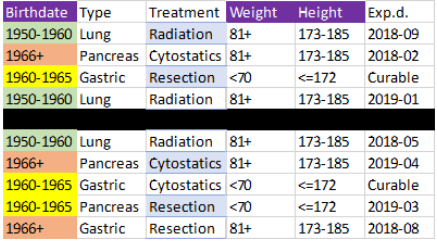
\includegraphics[width=0.6\textwidth]{Assignment0x07/image/anonimyzed_table}
	\caption{Anonymized Table}
	\label{img:anotable}
\end{figure}

\subsection{Explain the homogeneity attack against k-anonymized datasets. Can this be applied to your anonymized dataset? Explain your answer.}

\textbf{Homogeneity Attack}: If all members of a group of k records have the same sensitive data in a column, an attacker can find out that value despite anonymization (it’s always the same, thus predictable). This is hard to avoid completely - our 1950-1960 age group is extremely similar in nearly all respects; thus, an attacker will find out they have lung cancer and are receiving radiation treatment. 
